\title{\LaTeX Template}
\author{
        Kia Rahmani \\
                Department of Computer Science\\
        Purdue University, USA
}
\date{\today}

% Main Document
\documentclass[12pt,letter]{article}
\usepackage{xcolor,listings}
\usepackage{graphicx}
\usepackage[inline]{enumitem}
\usepackage[utf8]{inputenc}
\usepackage[english,ngerman]{babel}
\usepackage{amsmath}
\usepackage{mathtools}
\usepackage{mathpartir}

\begin{document}
\selectlanguage{english}
%\maketitle
%\begin{abstract} \end{abstract}


% Sections
% ---------------------------------------------------
\section{Three Languages}
\paragraph{}
In this document, I will introduce three abstraction levels for database programs, 
where each of which will be used at a  different stage of our final compilation process. 
The first and the last abstraction levels, capture the source (L1 or SQL) and the target 
(L3 or NoSQL) programs respectively. 
%
I have also included another language (L2) in between, that abstracts away implementation details 
and database specific features present in L3, 
allowing the managable comiler  for detecting detecting anomalies and rewriting
the programs on a generic key-value interface. 
This sepeartion also allows us to form a road map on
designing the final tool, focusing on (fundamentally) different challenges at each step and
offering different levels of formal robustness guarantees for each
transformation phase.


% Three Abstraction Levels
\begin{figure}[h]
\begin{center}
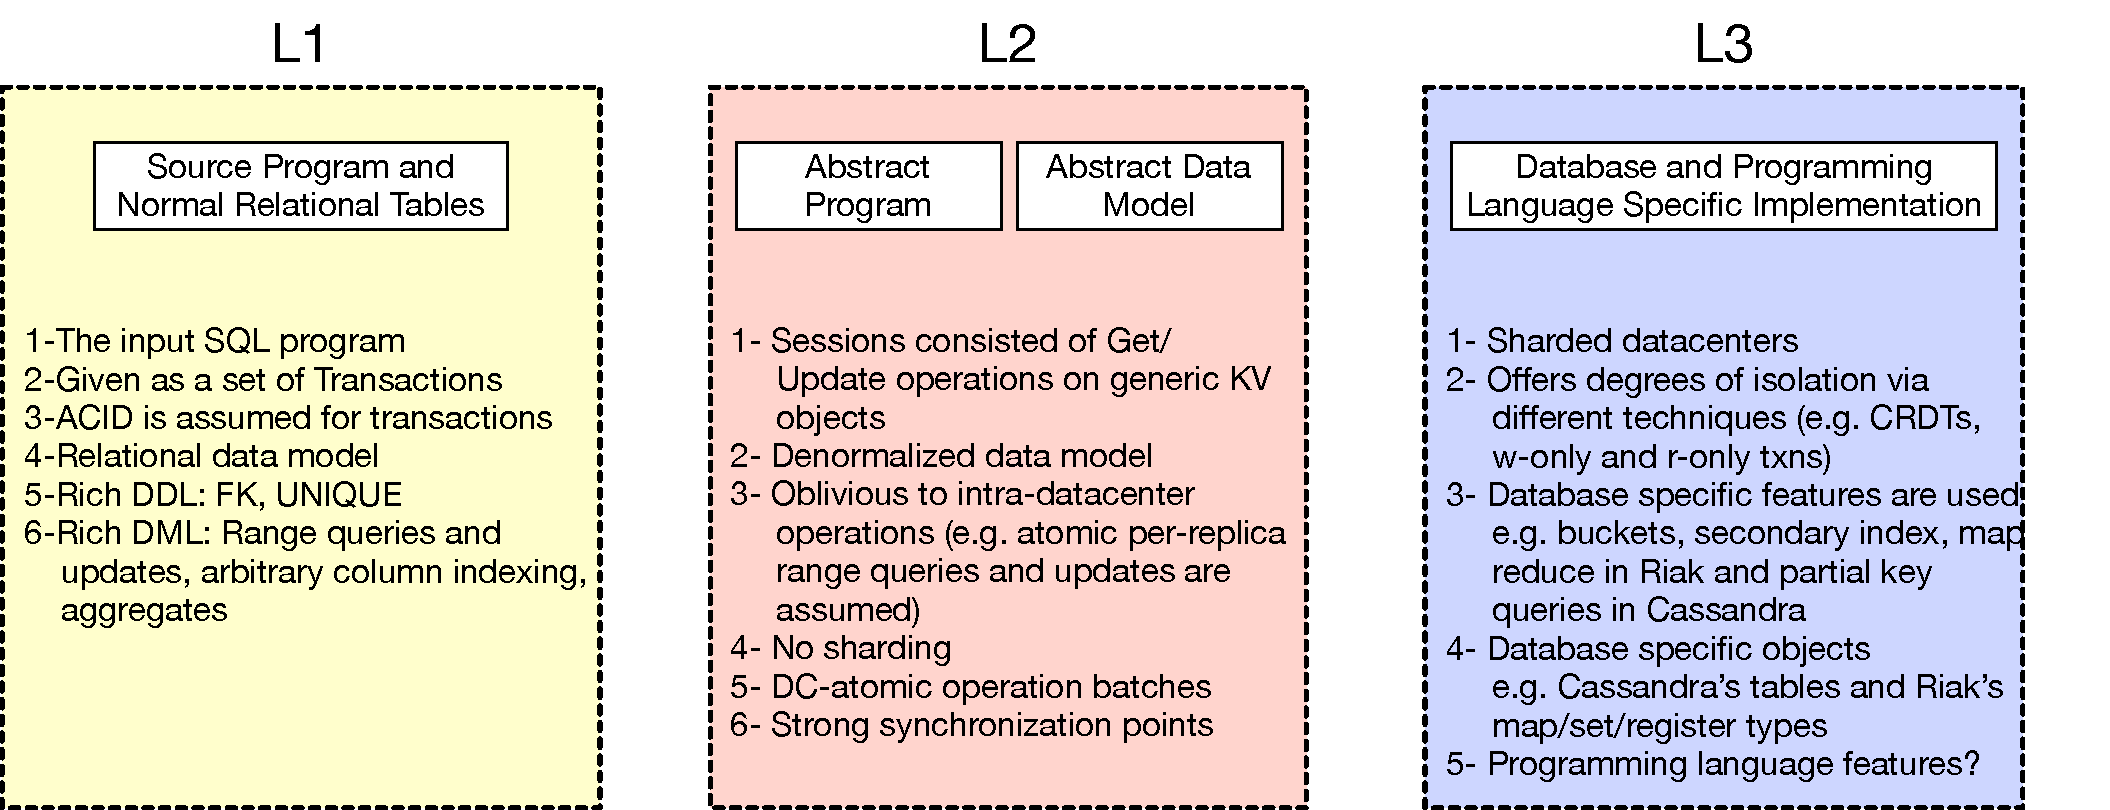
\includegraphics[width=\textwidth]{figures/levels.pdf}
\end{center}
\caption {Different Abstraction Levels}
\end{figure}

\paragraph{L1:}
The first abstraction level contains the source program which we assume is a 
traditional RDBMS backed program. 
The language covers interesting SQL queries (including range and join
queries) wrapped in loops or conditional statements. 
The syntax is fairly straightforward and is introduced in Kartik's document. 
\paragraph{L2:}
The next abstraction level is L2, which presents a generic key-value store interface and applications.
At this level we assume a replicated data store where each replica is a
stand-alone and complete copy of all data present in the global state (similar
to existing papers in the literature \cite{quelea,bolton,rdt}). 
As a result, L2 programs are oblivous to intra-datacenter actions, which
makes the departure from L1's model much more easier. 
For example, in L2 we assume atomic and isolated 
range queries and updates are already offered. However, in a
sharded database such operations add non-trivial and
database-specific challenges during the implementation phase. 

By abstracting the implementation details away, we can focus on the core of the
possible 
consistency and isolation anomalies in L2 and incrementally inject our programs with 
orchestration and synchronization points which will later be transformed into
concrete program code (L3). 

In L2 we assume key-value store operations could be packed together as batches
of operations that are guaranteed to execute atomically at either \emph{a single
datacenter level} or  \emph{globally}. Globally atomic batches are similar to
traditional ACID transactions which require unavailable synchronization points
in the program and may contain some program logic as well. On the other hand, DC-atomic batches guarantee isolated and
atomaic execution of the operations \emph{only in a single datacenter} and can be
offered by a partition-tolerant system. Note that at this level we simply
annotate the program with atomicity guards and do not consider specific 
databases or any specific implementation method. 
For example, a DC-atomic batch of operations in L2 could
be realized via multiple techniques in L3 such as Cassandra's atomic row updates,
Riak's CRDTs, Antidote's HAT transactions or even a naive implementation that
uses an external strong synchronization system.
\paragraph{L3:} The final abstraction level represents the concrete implementation
of the NoSQL program. As mentioned before, at this level we assume specific
database features and concrete synchronization and orchestration algorithms.
Consequently, for any L2 annotated program, we can generate multiple L3 implementation (one
for Cassandra, one for riak and one for Antidote for example). The transformation from
L2 to L3 requires writing libraries for each database and correctness
guarantees (which we might want to omit for the upcoming paper, since offering a
generic low-level reasoning framework for these systems is probably a
challenging task).
I will dive deeper into this level in the next write-up.





% ---------------------------------------------------
\section{Syntax of L2}
This section presents the formal syntax of L2, which is based on L1
(Kartik's SQL language) but works on fine-grained denormalized objects (instead
of normalized relational tables) and offers generic key-value operations
$get$ and $put$. Most importantly, the syntax allows wrapping multiple
operaitons in DC-atomic batches and wrapping higher level commands in
globally atomic batches.


% the syntax of L2
\begin{figure}[h]
	$$ k \in \texttt{Key}  \qquad  v \in \texttt{Value}  \qquad x \in \texttt{Variable} \qquad 
 	f \in \texttt{FieldName}  $$
	$$ \odot \in \{<,\leq,=,>,\geq\} \qquad \oplus \in \{\cap,\cup\}$$
	$$
	\begin{matrix*}[l]
        	obj &  ::= & (f,f) \\
        	r &  ::= & (k,v) \\
		\phi  & ::= & f \odot v \;|\; \neg
		\phi \\
		e  & ::= & x \;|\; (k,v) \;|\; e \oplus e\\
		op   & ::= & obj.put(r,v) \quad
		|\quad x\leftarrow obj.get(\phi)  \\
		c   & ::=  &  B_{DC}(\overline{op})
		\;|\; x\leftarrow e \;|\;
		\\  & & \texttt{IF}\; \phi_c \;\texttt{THEN} \;c \;\texttt{ELSE}\; c \;|\;  c;c \;|\;
	        B_{G}(c) \;|\;
		\\  & & \texttt{FOREACH}\; r \;\texttt{IN} \; x \; \texttt{DO}\; c \;\texttt{END}
		
	\end{matrix*}
	$$
\caption{Syntax of L2}
\end{figure}
Each L2 object type is a tuple of fieldnames\footnote{Fieldnames might belong to 
different original tables in a denormalized model handling joins}
$f_1$ and $f_2$ (each representing a table column in
the original model) which basically sepcifies an object that holds value(s) of
$f_2$ for a given $f_1$.
For example \texttt{address\_by\_age} is an
object that is queriable by age of the employees and can return the
addresses of all emplyees that satisfy a given search criterion on the
age (including range queries). We also assume a unique k (taken from the
original table's PK) attached to
each value (comprising a \emph{record} together) that is returned by
each query on an object. 
The syntax also introduces two diffrent atomicity and isolation guards: 
\begin{enumerate*}[label=(\roman*)]
  \item The DC-atomic batch ($B_{DC}$), which wraps a number of 
	  operations (puts and gets) and guarantees their atomic and isolated
	  execution (i.e. RC is offered by them and RR is offered for them). 
  \item When the application cannot be \emph{fixed} by mere use of DC batches 
	  programmer can wrap parts of the code (DB operations and control flow
	  statements) in globally atomic and isolated batches\footnote{this is similar
	  to the classic notion of ACID transactions, but we use the term
	  transaction to refer to the input SQL transactions. For example, in
	  input transaction NewOrder, can be translated into an L2 prorgam with
  2 different DC batch and one extra global batch}.
\end{enumerate*}

We also allow range queries on keys captured by an argument $\phi$ in the get
method of the objects. The reason that we limit the abstraction to properties on
single a fieldname 
(instead of the general case of SQL), is that none of the OTS NoSQL data stores offer such
sophisticated queries as atomic operations. This means that any
low-level implementation of a given L2 abstract program show anomalies that can
only be fixed by techniques present at L2 (e.g. batches). Thus, we only consider
single fieldname range queries that are manually composed which allows the
compiler to detect and fix the possible anomalies regarding them.
Almost all\footnote{range queris specifying
conditions on multiple fieldnames (instead of literals) are omitted from L2.} queries expressable in SQL can be
rewritten as a sequence of operations in the inital L2 program. For example:
\begin{itemize}
	\item (\texttt{SELECT} $f_1$ \texttt{WHERE} $f_2 > 100$) is translated to:
		\subitem $ x \leftarrow (f_1\_by\_f2).get(f_2>100)$ 
		\subitem - - x will hold approproate records
		(keys, values of $f_1$)
		
	\item \texttt{SELECT}  $f_1,f_2$ \texttt{WHERE}  $f_3=True$
		\subitem $ x \leftarrow (f_1\_by\_f3).get(f_3=True)$ 
		\subitem $ y \leftarrow (f_2\_by\_f3).get(f_3=True)$ 
	\item \texttt{SELECT}  $f_1$ \texttt{WHERE}  $f_2<100 \; \texttt{AND} \;
		f_3=False$
		\subitem $ t_1 \leftarrow (f_1\_by\_f2).get(f_2<100)$ 
		\subitem $ t_2 \leftarrow (f_1\_by\_f3).get(f_3=False)$
		\subitem $x\leftarrow t_1\cap t_2$
\end{itemize}

% ---------------------------------------------------
\section {Full Compilation Outline}
In this section, I will present the outline of the final compiler tool
using the abstraction levels discussed above.
\begin{figure}[t]
\begin{center}
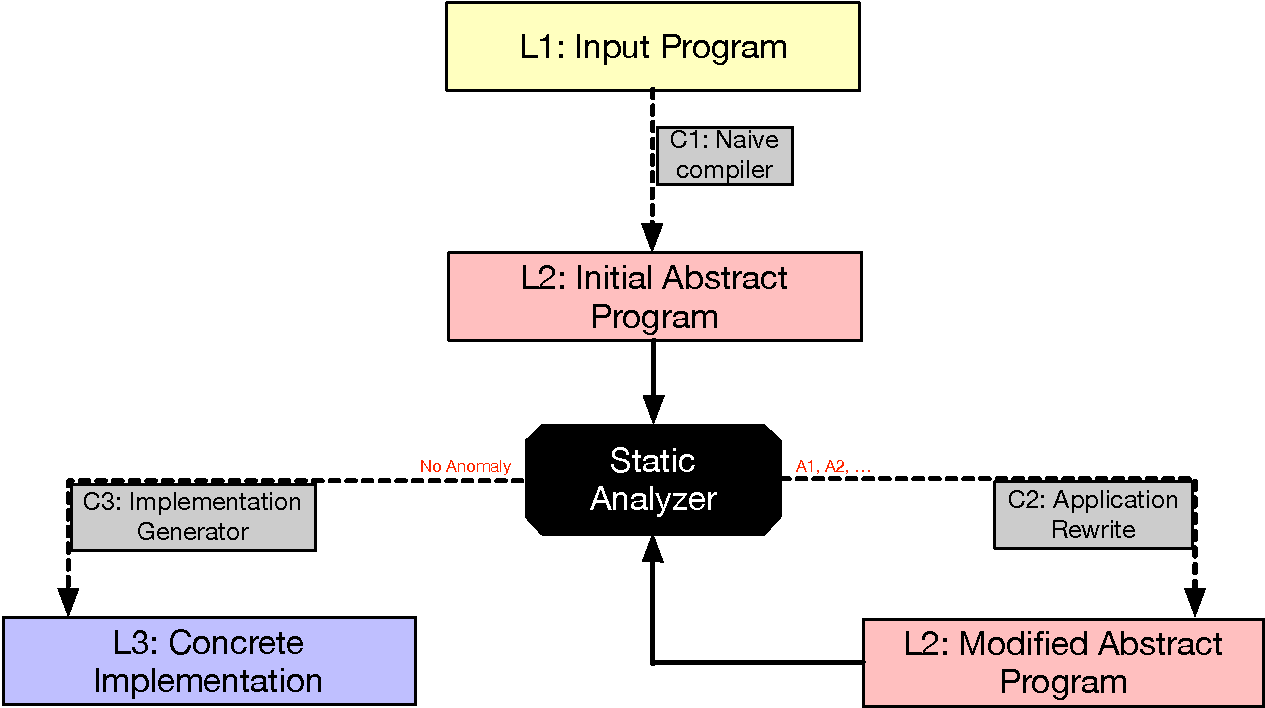
\includegraphics[width=\textwidth]{figures/outline.pdf}
\end{center}
\caption {Compilation Outline}
\label{fig:outline}
\end{figure}
Figure \ref{fig:outline} presents this outline, at the center of which we assume a
black box that analyzes L2 applications and returns a set of anomalies based on
Kartik's current tool. Since L2 is very similar to SQL, 
the design of this black box should be straightforward from what Kartik
already has; we just need to add the semantics for replication and batch
operations. 

The outline contains three different tools that generate/rewrite programs for
different target abstraction model: 
\begin{itemize}
	\item {\bf C1:} This is the very first compiler that is called only once
		and creates the initial version of L2 abstraction from the given
		L1 source program. We are almost done figuring out the details
		of this compiler (e.g. examples of the previous section are the
		most diffcult cases) and are ready to formally define 
		its operational semantics. 
		
		Next, we need to  define
		the operational semantics for L1 programs  and then based on the notion of eventual
		serializability\footnote{Breiefly, we require that the \emph{observable
		state} of
		an L2 program throughout an ES
		history should be equivalent to the states from a serial execution
	of the given transactions, following the notion of serializability
define in \cite{serforEC}}(ES) for
		L2 programs, we need to  
		prove that each ES execution of the initial L2 program is 
		\emph{equivalent} to the \emph{a serial execution} of
				the given L1 transactions. 	
	\item {\bf C2:} Trivially, not all executions of the initial L2 program are going
		to be ES, thus we need to incrementally alter the program by
		inserting DC and gloabl batch annotations to remove the detected
		anomalies from the set of possible executions of the L2 abstract
		program. We have already discussed the details of this step and
		how it works based on the anomalies that are detected. We will
		introduce the formal necessaties after defining the previous
		part.
	\item {\bf C3:} This is where our abstract key-value programs are
		concretized into real-world executable specific datastore
		programs. We can think about this compiler as plugable libraries
		that data store experts offer which guarantee the specified
		isolation and atomcity guarantees of L2. We are going to do it
		for one database (Antidote) but there is nothing stopping us
		from doing it for other databases as well. 
		We should discuss the level of formal vigorousness that we require 
		for this step. I believe, for our next paper this could be left 
		as a trusted base, since it is currently not clear to me how to formalize 
		the the low-level features used at this level. 


\end{itemize}













% The Biblography
\bibliographystyle{abbrv}
\bibliography{../kia-bib}
\end{document}
